% =============================================================================
%  Machine Learning for Petroleum Engineers Using Python
%  Clase 3: pandas y Carga de Datos --- Producción y Well Logs (Volve)
%  SLB Ecuador | UDLA
%
%  Compilar: pdflatex -shell-escape presentacion.tex (x2 para refs)
% =============================================================================
\documentclass[aspectratio=169, 11pt]{beamer}

% ── Codificación y lenguaje ──────────────────────────────────────────────────
\usepackage[T1]{fontenc}
\usepackage[utf8]{inputenc}
\usepackage[spanish,es-noshorthands]{babel}

% ── Fuentes ──────────────────────────────────────────────────────────────────
\usepackage{FiraSans}
\usepackage{FiraMono}
\renewcommand{\familydefault}{\sfdefault}

% ── Gráficos y diagramas ────────────────────────────────────────────────────
\usepackage{graphicx}
\usepackage{tikz}
\usetikzlibrary{arrows.meta, positioning, shapes.geometric, calc, fit, decorations.pathreplacing}
\usepackage{fontawesome5}

% ── Código fuente ────────────────────────────────────────────────────────────
\usepackage{minted}
\usepackage{tcolorbox}
\tcbuselibrary{minted, skins, breakable}

% ── Tablas y utilidades ──────────────────────────────────────────────────────
\usepackage{amsmath}
\usepackage{colortbl}
\usepackage{booktabs}
\usepackage{multicol}
\usepackage{hyperref}
\usepackage{calc}

% =============================================================================
%  PALETA DE COLORES (rojo UDLA + variantes)
% =============================================================================
\definecolor{arcaRed}{HTML}{C82B40}
\definecolor{arcaDark}{HTML}{6B1525}
\definecolor{udlaCrimson}{HTML}{A31545}
\definecolor{arcaGray}{HTML}{F5F5F5}
\definecolor{arcaLightGray}{HTML}{EBEBEB}
\definecolor{textDark}{HTML}{2D2D2D}
\definecolor{textMuted}{HTML}{6B7280}
\definecolor{codeGreen}{HTML}{16A34A}
\definecolor{codeBlue}{HTML}{2563EB}
\definecolor{codeOrange}{HTML}{EA580C}
\definecolor{slbBlue}{HTML}{0014DC}
\definecolor{terminalBg}{HTML}{0F172A}
\definecolor{terminalGreen}{HTML}{86EFAC}
\definecolor{terminalMuted}{HTML}{94A3B8}
\definecolor{codeBg}{HTML}{FAFAFA}

% =============================================================================
%  CONFIGURACIÓN DEL TEMA BEAMER
% =============================================================================
\usetheme{default}
\usecolortheme{default}

\setbeamertemplate{navigation symbols}{}
\setbeamertemplate{footline}{}
\setbeamertemplate{headline}{}

\setbeamercolor{normal text}{fg=textDark}
\setbeamercolor{frametitle}{fg=arcaRed, bg=white}
\setbeamercolor{title}{fg=white}
\setbeamercolor{subtitle}{fg=white!85}
\setbeamercolor{author}{fg=white!80}
\setbeamercolor{date}{fg=white!70}
\setbeamercolor{item}{fg=arcaRed}
\setbeamercolor{subitem}{fg=arcaDark}
\setbeamercolor{block title}{fg=white, bg=arcaRed}
\setbeamercolor{block body}{fg=textDark, bg=arcaGray}
\setbeamercolor{block title alerted}{fg=white, bg=codeOrange}
\setbeamercolor{block body alerted}{fg=textDark, bg=arcaGray}
\setbeamercolor{block title example}{fg=white, bg=codeGreen}
\setbeamercolor{block body example}{fg=textDark, bg=arcaGray}
\setbeamercolor{section in toc}{fg=arcaDark}

\setbeamerfont{frametitle}{size=\Large, series=\bfseries}
\setbeamerfont{title}{size=\huge, series=\bfseries}
\setbeamerfont{subtitle}{size=\large}
\setbeamerfont{author}{size=\normalsize}
\setbeamerfont{date}{size=\small}
\setbeamerfont{block title}{size=\normalsize, series=\bfseries}
\setbeamerfont{footnote}{size=\tiny}

\setbeamertemplate{itemize item}{\scriptsize\raise1.5pt\hbox{\color{arcaRed}$\blacktriangleright$}}
\setbeamertemplate{itemize subitem}{\scriptsize\raise1pt\hbox{\color{arcaDark}$\bullet$}}
\setbeamertemplate{enumerate items}[default]
\setbeamercolor{enumerate item}{fg=arcaRed}

% =============================================================================
%  HEADER
% =============================================================================
\setbeamertemplate{headline}{%
  \begin{tikzpicture}[remember picture, overlay]
    \fill[arcaDark] (current page.north west) rectangle
      ([yshift=-0.7cm]current page.north east);
    \node[anchor=west, inner sep=0pt] at
      ([xshift=0.6cm, yshift=-0.35cm]current page.north west)
      {
\includegraphics[height=0.45cm]{../logo_udla_white.png}};
    \node[anchor=east, inner sep=0pt] at
      ([xshift=-0.6cm, yshift=-0.35cm]current page.north east)
      {
\includegraphics[height=0.42cm]{../SLB_white.png}};
  \end{tikzpicture}%
  \vspace{0.7cm}%
}

% =============================================================================
%  FOOTER
% =============================================================================
\setbeamertemplate{footline}{%
  \begin{tikzpicture}[remember picture, overlay]
    \draw[arcaLightGray, line width=0.4pt]
      ([yshift=0.55cm, xshift=0.6cm]current page.south west) --
      ([yshift=0.55cm, xshift=-0.6cm]current page.south east);
    \node[anchor=south, font=\tiny\color{textMuted}] at
      ([yshift=0.15cm]current page.south)
      {Machine Learning for Petroleum Engineers Using Python \(\cdot\) SLB Ecuador};
    \node[anchor=south east, font=\scriptsize\bfseries\color{arcaRed}] at
      ([xshift=-0.6cm, yshift=0.15cm]current page.south east)
      {\insertframenumber};
  \end{tikzpicture}%
}

% =============================================================================
%  FRAMETITLE personalizado con línea roja
% =============================================================================
\setbeamertemplate{frametitle}{%
  \vspace{0.25cm}%
  \usebeamerfont{frametitle}\usebeamercolor[fg]{frametitle}\insertframetitle%
  \par\vspace{2pt}%
  \begin{tikzpicture}
    \fill[arcaRed] (0,0) rectangle (3cm, 1.5pt);
    \fill[arcaLightGray] (3cm,0) rectangle (\textwidth, 0.5pt);
  \end{tikzpicture}%
  \vspace{0.1cm}%
}

% =============================================================================
%  ESTILO DE BLOQUES DE CÓDIGO (minted + tcolorbox)
% =============================================================================
\newtcblisting{pyblock}[1][]{%
  listing engine=minted,
  minted language=python,
  minted style=xcode,
  minted options={
    fontsize=\small,
    linenos=false,
    breaklines=true,
    python3=true
  },
  enhanced,
  colback=codeBg,
  colframe=arcaRed,
  left=8pt,
  right=6pt,
  top=5pt,
  bottom=5pt,
  boxrule=0pt,
  leftrule=3pt,
  arc=3pt,
  listing only,
  title={\hspace{-2pt}\faPython\hspace{5pt}Python},
  fonttitle=\scriptsize\bfseries,
  colbacktitle=arcaRed,
  coltitle=white,
  attach boxed title to top left={xshift=8pt, yshift=-7pt},
  boxed title style={
    arc=2pt, boxrule=0pt,
    top=1.5pt, bottom=1.5pt, left=6pt, right=6pt
  },
  drop fuzzy shadow=black!12,
  #1
}

\newtcblisting{outputblock}[1][]{%
  listing engine=minted,
  minted language=text,
  minted style=bw,
  minted options={
    fontsize=\small,
    breaklines=true,
    formatcom=\color{terminalGreen}
  },
  enhanced,
  colback=terminalBg,
  colframe=terminalBg,
  coltext=terminalGreen,
  left=10pt, right=6pt, top=5pt, bottom=5pt,
  boxrule=0pt,
  arc=3pt,
  listing only,
  title={\hspace{-2pt}\faTerminal\hspace{5pt}Output},
  fonttitle=\scriptsize\bfseries,
  colbacktitle=terminalGreen!85!black,
  coltitle=terminalBg,
  attach boxed title to top left={xshift=8pt, yshift=-7pt},
  boxed title style={
    arc=2pt, boxrule=0pt,
    top=1.5pt, bottom=1.5pt, left=6pt, right=6pt
  },
  #1
}

% =============================================================================
%  SECTION DIVIDERS
% =============================================================================
\newcommand{\sectionframe}[2]{%
  \begingroup
    \setbeamertemplate{headline}{}
    \setbeamertemplate{footline}{}
    \setbeamertemplate{navigation symbols}{}
    \begin{frame}[plain, noframenumbering]
      \begin{tikzpicture}[remember picture, overlay]
        \fill[arcaRed] (current page.south west) rectangle (current page.north east);
        \node[anchor=center, text=white, font=\Huge\bfseries, text width=12cm,
              align=center] at ([yshift=0.5cm]current page.center) {#1};
        \node[anchor=center, text=white!80, font=\large, text width=10cm,
              align=center] at ([yshift=-0.8cm]current page.center) {#2};
      \end{tikzpicture}
    \end{frame}
  \endgroup
}

% =============================================================================
%  METADATOS
% =============================================================================
\title{Machine Learning for Petroleum Engineers\\Using Python}
\subtitle{Módulo 3 · Clase 1: Regresión Lineal --- Tu Primer Modelo Predictivo}
\author{Carlos Enrique Mosquera Trujillo}
\date{2026}

% =============================================================================
%  DOCUMENTO
% =============================================================================
% =============================================================================
%  DOCUMENTO
% =============================================================================
\begin{document}

% ─────────────────────────────────────────────────────────────────────────────
%  PORTADA
% ─────────────────────────────────────────────────────────────────────────────
{
\setbeamertemplate{headline}{}
\setbeamertemplate{footline}{}
\begin{frame}[plain, noframenumbering]
  \begin{tikzpicture}[remember picture, overlay]
    \fill[white] (current page.south west) rectangle (current page.north east);
    \fill[arcaRed] (current page.north west) rectangle ([yshift=-0.35cm]current page.north east);
    \fill[arcaDark] (current page.south west) rectangle ([yshift=0.35cm]current page.south east);
    \fill[arcaRed]
      ([xshift=1.1cm, yshift=-0.35cm]current page.north west) rectangle
      ([xshift=1.15cm, yshift=0.35cm]current page.south west);
    \node[anchor=north west, inner sep=0pt] at
      ([xshift=1.8cm, yshift=-1.2cm]current page.north west)
      {
\includegraphics[height=1.6cm]{../logo_udla.png}};
    \node[anchor=north east, inner sep=0pt] at
      ([xshift=-1.5cm, yshift=-1.2cm]current page.north east)
      {
\includegraphics[height=1.5cm]{../SLB.png}};
    \node[anchor=center, text=arcaDark, text width=14.5cm, align=center] at
      ([yshift=0.95cm]current page.center) {
        {\LARGE\bfseries Machine Learning for Petroleum Engineers}\\[8pt]
        {\LARGE\bfseries Using Python}
      };
    \fill[arcaRed]
      ([yshift=-0.35cm, xshift=-3.2cm]current page.center) rectangle
      ([yshift=-0.28cm, xshift=3.2cm]current page.center);
    \node[anchor=center, text=arcaRed, font=\large, text width=13cm, align=center] at
      ([yshift=-1.3cm]current page.center) {
        Módulo 3 · Clase 1\\[3pt]
        Regresión Lineal: Tu Primer Modelo Predictivo
      };
    \node[anchor=center, text=textMuted, font=\normalsize] at
      ([yshift=-2.3cm]current page.center) {
        {\color{arcaRed}\faUser}\hspace{6pt}Carlos Enrique Mosquera Trujillo
        \hspace{16pt}
        {\color{arcaRed}\faIndustry}\hspace{4pt}SLB Ecuador
      };
  \end{tikzpicture}
\end{frame}
}

% ─────────────────────────────────────────────────────────────────────────────
%  RECAP + HOJA DE RUTA

\begin{frame}{Empieza el Módulo de Machine Learning}
  \vspace{-6pt}
  \begin{columns}[T]
    \begin{column}{0.48\textwidth}
      {\small\color{arcaDark}\bfseries\faCheckCircle\hspace{5pt}Hasta ahora:}
      \vspace{4pt}
      {\footnotesize\color{textMuted}
      \begin{itemize}\setlength{\itemsep}{3pt}
        \item[{\color{codeGreen}\scriptsize\faCheck}]
          Módulo 1: Python y carga de datos (pandas, CSV, LAS)
        \item[{\color{codeGreen}\scriptsize\faCheck}]
          Módulo 2: exploración y limpieza (EDA)
        \item[{\color{codeGreen}\scriptsize\faCheck}]
          Sabemos \textbf{describir} los datos: media, correlación, gráficos
      \end{itemize}
      }
      \vspace{8pt}
      {\scriptsize\color{textMuted}\itshape
        Describir contesta ``¿qué pasó?''.
        Hoy damos el salto a ``¿qué \textbf{va} a pasar?''.}
    \end{column}
    \begin{column}{0.48\textwidth}
      {\small\color{arcaDark}\bfseries\faForward\hspace{5pt}Hoy (Clase 1 de ML):}
      \vspace{4pt}
      {\footnotesize\color{textMuted}
      \begin{itemize}\setlength{\itemsep}{3pt}
        \item[{\color{arcaRed}\scriptsize\faArrowRight}]
          Qué es \textbf{predecir} y qué es un \textbf{modelo}
        \item[{\color{arcaRed}\scriptsize\faArrowRight}]
          La \textbf{regresión lineal}: la recta que mejor se ajusta
        \item[{\color{arcaRed}\scriptsize\faArrowRight}]
          Cómo medir si el modelo es \textbf{bueno} (R\textsuperscript{2}, RMSE)
        \item[{\color{arcaRed}\scriptsize\faArrowRight}]
          Muchas variables, estandarización y \textbf{train/test}
      \end{itemize}
      }
      \vspace{6pt}
      {\scriptsize\color{arcaDark}\itshape
        Reto real: \textbf{reconstruir un registro de pozo} a partir de otros.}
    \end{column}
  \end{columns}
\end{frame}


\begin{frame}[shrink=10]{¿Qué es Machine Learning?}
  \vspace{-6pt}
  {\small\color{arcaDark}\bfseries
    Un cambio de enfoque: en vez de escribir la regla, dejamos que el computador la \textbf{aprenda} de los ejemplos.}

  \vspace{10pt}
  \begin{columns}[T]
    \begin{column}{0.48\textwidth}
      \begin{tcolorbox}[colback=arcaGray, colframe=textMuted, boxrule=0pt, leftrule=3pt,
        arc=3pt, left=6pt, right=6pt, top=5pt, bottom=5pt]
        {\scriptsize\color{textDark}\bfseries\faCode\hspace{4pt}Programación clásica}\\[4pt]
        {\scriptsize\color{textMuted}
          El humano escribe la regla:\\[2pt]
          \texttt{si presion > 3000: alerta}\\[4pt]
          Funciona cuando la regla \textbf{se conoce}
          y se puede escribir a mano.}
      \end{tcolorbox}
    \end{column}
    \begin{column}{0.48\textwidth}
      \begin{tcolorbox}[colback=arcaGray, colframe=arcaRed, boxrule=0pt, leftrule=3pt,
        arc=3pt, left=6pt, right=6pt, top=5pt, bottom=5pt]
        {\scriptsize\color{arcaRed}\bfseries\faRobot\hspace{4pt}Machine Learning}\\[4pt]
        {\scriptsize\color{textMuted}
          Le damos \textbf{ejemplos con la respuesta}
          y el computador \textbf{encuentra la regla}
          que mejor los explica.\\[4pt]
          Funciona cuando la regla es demasiado
          compleja para escribirla a mano.}
      \end{tcolorbox}
    \end{column}
  \end{columns}

  \vspace{10pt}
  {\footnotesize\color{textMuted}
  \begin{itemize}\setlength{\itemsep}{4pt}
    \item[{\color{arcaRed}\scriptsize\faArrowRight}]
      Hoy hacemos aprendizaje \textbf{supervisado}: aprender de ejemplos que
      \textbf{ya traen la respuesta correcta}.
    \item[{\color{arcaRed}\scriptsize\faArrowRight}]
      Y dentro de lo supervisado, \textbf{regresión}: la respuesta que buscamos
      es \textbf{un número} (el valor del sónico).
  \end{itemize}
  }
\end{frame}

\begin{frame}{El Problema Real de Hoy: un Sensor que Falla}
  \vspace{-6pt}
  {\small\color{arcaDark}\bfseries
    El sensor que mide el registro sónico se dañó a mitad del pozo. Hay un tramo \textbf{sin datos}.}

  \vspace{6pt}
  \begin{columns}[T]
    \begin{column}{0.54\textwidth}
      {\footnotesize\color{textMuted}
      \begin{itemize}\setlength{\itemsep}{7pt}
        \item[{\color{arcaRed}\scriptsize\faDollarSign}]
          Volver a correr la herramienta significa traer de nuevo la
          unidad de registro y \textbf{parar el pozo}: días de equipo y
          \textbf{cientos de miles de dólares}.
        \item[{\color{arcaRed}\scriptsize\faExclamationTriangle}]
          A veces ni siquiera se puede: el pozo ya está entubado.
        \item[{\color{codeGreen}\scriptsize\faLightbulb}]
          \textbf{Decisión de negocio:} ¿pagamos por re-loguear, o
          \textbf{confiamos en un modelo} que reconstruya el sónico a
          partir de los sensores que \textbf{sí} funcionaron?
      \end{itemize}
      }
    \end{column}
    \begin{column}{0.43\textwidth}
      \begin{tcolorbox}[colback=arcaGray, colframe=arcaRed, boxrule=0pt,
        leftrule=3pt, arc=3pt, left=6pt, right=6pt, top=5pt, bottom=5pt]
        {\scriptsize\color{arcaDark}\bfseries La apuesta:}\\[4pt]
        {\scriptsize\color{textMuted}
        aprender de los tramos donde \textbf{sí} tenemos las tres medidas
        (sónico, densidad, porosidad) para \textbf{rellenar} donde el
        sensor falló --- sin gastar en re-loguear.}
      \end{tcolorbox}
      \vspace{5pt}
      {\scriptsize\color{textMuted}\itshape
        Es un problema real de la industria; hay papers prediciendo el
        sónico del campo Volve exactamente así.}
    \end{column}
  \end{columns}
\end{frame}

%% ═════════════════════════════════════════════════════════════════════════════
\sectionframe{La Gran Idea}{Relaciones entre variables que podemos modelar}
% ═════════════════════════════════════════════════════════════════════════════
\begin{frame}[shrink=8]{Ustedes Ya Piensan en Relaciones}
  \vspace{-6pt}
  {\small\color{arcaDark}\bfseries
    Nadie llega en blanco: en la operación diaria ustedes ya predicen usando relaciones.}

  \vspace{8pt}
  {\footnotesize\color{textMuted}
  \begin{itemize}\setlength{\itemsep}{7pt}
    \item[{\color{arcaRed}\scriptsize\faArrowDown}]
      A más \textbf{profundidad} \(\to\) más \textbf{presión} y más \textbf{temperatura}.
    \item[{\color{arcaRed}\scriptsize\faClock}]
      Más \textbf{horas de bomba} \(\to\) más \textbf{consumo de diésel}.
    \item[{\color{arcaRed}\scriptsize\faTint}]
      Más \textbf{agua} en el fluido \(\to\) más \textbf{costo de tratamiento}.
  \end{itemize}
  }

  \vspace{8pt}
  \centering
  \begin{tcolorbox}[colback=arcaGray, colframe=arcaRed, boxrule=0pt, leftrule=3pt,
    arc=3pt, left=8pt, right=8pt, top=6pt, bottom=6pt, width=0.86\textwidth]
    {\footnotesize\color{arcaDark}\itshape
      ``Si el pozo está a 4\,000 m, espera unos \(120\,^{\circ}\)C.''}\\[3pt]
    {\scriptsize\color{textMuted}
      Eso es una \textbf{predicción} --- hecha de memoria, con una
      \textbf{relación entre dos variables} que ustedes ya conocen.}
  \end{tcolorbox}

  \vspace{6pt}
  {\footnotesize\color{arcaDark}
    Hoy haremos exactamente eso mismo, pero \textbf{preciso, repetible y auditable}.}
\end{frame}

\begin{frame}{¿Qué es una Relación entre Dos Variables?}
  \vspace{-6pt}
  {\small\color{arcaDark}\bfseries
    Una \textbf{variable} es algo que medimos y que cambia. Hay \textbf{relación} cuando
    conocer una nos dice algo de la otra.}

  \vspace{8pt}
  \begin{columns}[T]
    \begin{column}{0.48\textwidth}
      \begin{tcolorbox}[colback=arcaGray, colframe=codeGreen, boxrule=0pt, leftrule=3pt,
        arc=3pt, left=6pt, right=6pt, top=5pt, bottom=5pt]
        {\scriptsize\color{codeGreen}\bfseries\faCheck\hspace{4pt}SÍ hay relación}\\[4pt]
        {\scriptsize\color{textMuted}
          \textbf{Profundidad y temperatura.} Si me dicen ``4\,000 m'', ya \textbf{no}
          espero \textit{cualquier} temperatura: espero una zona estrecha de valores.
          Saber una me \textbf{acerca} a la otra.}
      \end{tcolorbox}
    \end{column}
    \begin{column}{0.48\textwidth}
      \begin{tcolorbox}[colback=arcaGray, colframe=arcaRed, boxrule=0pt, leftrule=3pt,
        arc=3pt, left=6pt, right=6pt, top=5pt, bottom=5pt]
        {\scriptsize\color{arcaRed}\bfseries\faTimes\hspace{4pt}NO hay relación}\\[4pt]
        {\scriptsize\color{textMuted}
          \textbf{Día de la semana y densidad de la roca.} Saber que hoy es martes
          no me acerca \textbf{en nada} al valor de la densidad. Conocer una
          no dice nada de la otra.}
      \end{tcolorbox}
    \end{column}
  \end{columns}

  \vspace{12pt}
  \centering
  {\footnotesize\color{arcaDark}
    \faLightbulb[regular]\hspace{4pt}\textbf{Test de bolsillo:}
    ¿saber \(A\) me ayuda a adivinar \(B\)?\quad
    Si la respuesta es sí, hay una relación que podemos \textbf{aprovechar}.}
\end{frame}

\begin{frame}{La Relación de Hoy, Dibujada}
  \vspace{-6pt}
  {\small\color{arcaDark}\bfseries
    Dos mediciones del pozo: densidad (\texttt{DEN}) y sónico (\texttt{AC}). Un punto por profundidad.}

  \vspace{4pt}
  \begin{columns}[T]
    \begin{column}{0.52\textwidth}
      \centering
      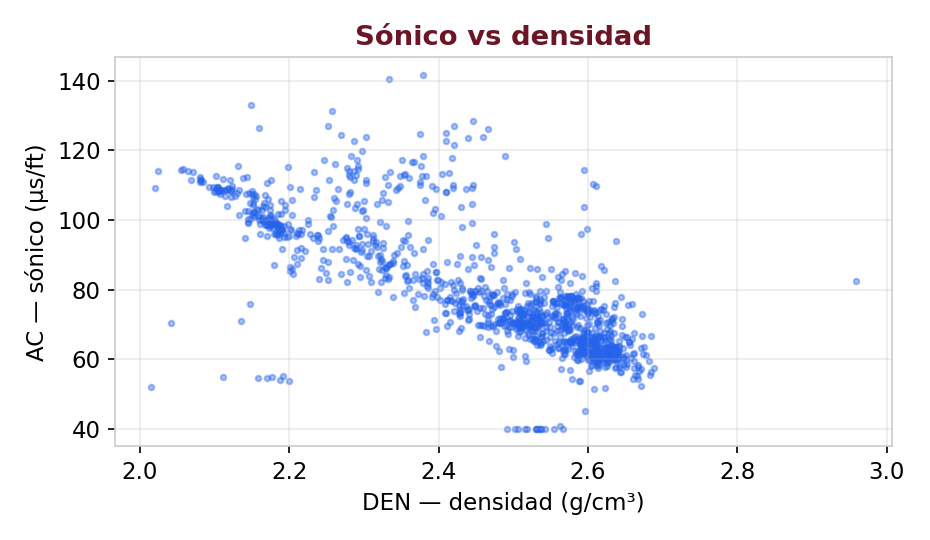
\includegraphics[width=\textwidth]{fig_explora_scatter.png}
    \end{column}
    \begin{column}{0.44\textwidth}
      {\footnotesize\color{textMuted}
      \begin{itemize}\setlength{\itemsep}{6pt}
        \item[{\color{arcaRed}\scriptsize\faArrowRight}]
          Cada punto es \textbf{una profundidad} del pozo (hay 6\,893).
        \item[{\color{arcaRed}\scriptsize\faArrowRight}]
          La nube \textbf{no es redonda: está inclinada}.
          Inclinada = hay relación.
        \item[{\color{arcaRed}\scriptsize\faArrowRight}]
          Léanla: roca más densa \(\to\) el sonido viaja más rápido
          \(\to\) sónico más bajo.
        \item[{\color{codeGreen}\scriptsize\faQuestion}]
          La pregunta del día: ¿es \textbf{lo bastante firme} para
          rellenar el tramo del sensor dañado?
      \end{itemize}
      }
    \end{column}
  \end{columns}
\end{frame}

\begin{frame}[shrink=10]{Ponerle Número a la Relación: la Correlación}
  \vspace{-6pt}
  {\small\color{arcaDark}\bfseries
    La correlación responde \textbf{dos preguntas} con un solo número entre \(-1\) y \(+1\).}

  \vspace{6pt}
  {\footnotesize\color{textMuted}
  \begin{itemize}\setlength{\itemsep}{4pt}
    \item[{\color{arcaRed}\bfseries 1.}]
      \textbf{¿En qué dirección va?} El \textbf{signo}: con \(+\), cuando una crece la otra
      tiende a crecer; con \(-\), cuando una crece la otra tiende a caer.
    \item[{\color{arcaRed}\bfseries 2.}]
      \textbf{¿Qué tan firme es?} La \textbf{cercanía a \(\pm 1\)}: cerca de \(\pm 1\) la nube es
      casi una línea (saber una casi fija la otra); cerca de \(0\), la nube es redonda
      (saber una no ayuda).
  \end{itemize}
  }

  \vspace{10pt}
  \centering
  \begin{tikzpicture}[font=\scriptsize]
    \draw[arcaRed, line width=1.4pt] ({-0.755*6},0.12) -- ({-0.755*6},0.75);
    \node[above, text=arcaRed, font=\tiny\bfseries] at ({-0.755*6},0.75) {DEN $=-0.76$};
    \draw[codeBlue, line width=1.4pt] ({0.725*6},0.12) -- ({0.725*6},0.75);
    \node[above, text=codeBlue, font=\tiny\bfseries] at ({0.725*6},0.75) {NEU $=+0.72$};
    \draw[textMuted, line width=1.2pt] ({-0.101*6},0.12) -- ({-0.101*6},0.50);
    \node[above, text=textMuted, font=\tiny\bfseries] at ({-0.101*6},0.50) {RDEP};
    \draw[line width=1.2pt, arcaLightGray] (-6,0) -- (6,0);
    \foreach \x/\v in {-6/-1, -3/-0.5, 0/0, 3/0.5, 6/1}{
      \draw[line width=1pt, textMuted] (\x,0.12) -- (\x,-0.12);
      \node[below, text=textDark, font=\scriptsize\bfseries] at (\x,-0.18) {\v};
    }
    \node[below, text=arcaRed, font=\tiny\bfseries] at (-4.5,-0.55) {fuerte y negativa};
    \node[below, text=textMuted, font=\tiny\bfseries] at (0,-0.55) {débil};
    \node[below, text=codeBlue, font=\tiny\bfseries] at (4.5,-0.55) {fuerte y positiva};
  \end{tikzpicture}

  \vspace{10pt}
  {\scriptsize\color{textMuted}
    \faLightbulb[regular]\hspace{3pt}%
    Regla de bolsillo del curso: \(|r|>0.7\) fuerte \(\cdot\) 0.3--0.7 media \(\cdot\) \(<0.3\) débil.
    Nuestra pareja \texttt{DEN}--\texttt{AC} da \textbf{\(-0.76\)}: fuerte y negativa.}
\end{frame}

\begin{frame}{¿Qué Significa que una Relación sea Lineal?}
  \vspace{-6pt}
  {\small\color{arcaDark}\bfseries
    Lineal = la relación es \textbf{pareja}: el mismo paso en una variable produce
    \textbf{siempre el mismo} paso en la otra.}

  \vspace{6pt}
  \begin{columns}[T]
    \begin{column}{0.52\textwidth}
      {\footnotesize\color{textMuted}
      \begin{itemize}\setlength{\itemsep}{7pt}
        \item[{\color{arcaRed}\scriptsize\faDollarSign}]
          \textbf{Tanquear el carro}: el galón 1 cuesta lo mismo que el galón 10.
          Por eso el total es precio \(\times\) galones: \textbf{una recta}.
        \item[{\color{arcaRed}\scriptsize\faArrowDown}]
          \textbf{Presión hidrostática}: cada 100 m de profundidad suman
          \(\approx\) la misma presión, arriba o abajo del pozo.
        \item[{\color{codeGreen}\scriptsize\faCheck}]
          Si el paso vale \textbf{siempre lo mismo}, el dibujo de la relación
          es una \textbf{línea recta}.
      \end{itemize}
      }
    \end{column}
    \begin{column}{0.44\textwidth}
      \centering
      \begin{tikzpicture}[font=\tiny, scale=0.9]
        \draw[-{Stealth[length=4pt]}, textMuted] (0,0) -- (5.2,0) node[below left, font=\tiny] {galones};
        \draw[-{Stealth[length=4pt]}, textMuted] (0,0) -- (0,3.4) node[below left, rotate=90, font=\tiny] {};
        \node[left, font=\tiny, text=textMuted, rotate=90, anchor=south] at (-0.25,1.6) {total \$};
        \draw[arcaRed, line width=1.8pt] (0.2,0.25) -- (4.9,3.05);
        % paso 1
        \draw[dashed, textMuted] (1.0,0.73) -- (1.8,0.73) -- (1.8,1.20);
        \node[below, text=textDark] at (1.4,0.71) {+1};
        \node[right, text=arcaRed, font=\tiny\bfseries] at (1.8,0.95) {+m};
        % paso 2 (mismo tamano)
        \draw[dashed, textMuted] (3.2,2.04) -- (4.0,2.04) -- (4.0,2.51);
        \node[below, text=textDark] at (3.6,2.02) {+1};
        \node[right, text=arcaRed, font=\tiny\bfseries] at (4.0,2.26) {+m};
        \node[below, text=arcaDark, font=\tiny\bfseries, align=center] at (2.6,-0.42)
          {el paso vale lo mismo aquí y allá};
      \end{tikzpicture}
    \end{column}
  \end{columns}

  \vspace{6pt}
  {\scriptsize\color{textMuted}
    \faLightbulb[regular]\hspace{3pt}%
    A ese ``precio del paso'' lo llamaremos \textbf{pendiente} (\(m\)). Es el corazón de la recta.}
\end{frame}

\begin{frame}{La Relación, Escrita como Fórmula}
  \vspace{-6pt}
  {\small\color{arcaDark}\bfseries
    Si el paso siempre vale lo mismo, la relación completa cabe en una línea de álgebra.}

  \vspace{10pt}
  \centering
  {\large\color{arcaDark}
  \(
    \underbrace{\texttt{AC}}_{\text{predicción}}
    \;=\;
    \underbrace{b}_{\substack{\text{intercepto}\\ \text{(dónde arranca)}}}
    \;+\;
    \underbrace{m}_{\substack{\text{pendiente}\\ \text{(precio del paso)}}}
    \;\times\;
    \underbrace{\texttt{DEN}}_{\text{dato conocido}}
  \)
  }

  \vspace{12pt}
  {\footnotesize\color{textMuted}
  \begin{itemize}\setlength{\itemsep}{5pt}
    \item[{\color{arcaRed}\scriptsize\faArrowRight}]
      \(m\) (\textbf{pendiente}): cuánto cambia el sónico por cada \(+1\) de densidad.
    \item[{\color{arcaRed}\scriptsize\faArrowRight}]
      \(b\) (\textbf{intercepto}): el punto de arranque de la recta.
    \item[{\color{codeGreen}\scriptsize\faCheck}]
      \textbf{``Entrenar el modelo''} = encontrar los mejores \(m\) y \(b\) para nuestros
      datos. Eso lo hace el computador en un segundo.
  \end{itemize}
  }
\end{frame}

\begin{frame}{No Todas las Relaciones Son Parejas}
  \vspace{-6pt}
  {\small\color{arcaDark}\bfseries
    En el mundo real, muchas relaciones existen y son claras\ldots pero \textbf{no} son rectas.}

  \vspace{4pt}
  \begin{columns}[T]
    \begin{column}{0.55\textwidth}
      \centering
      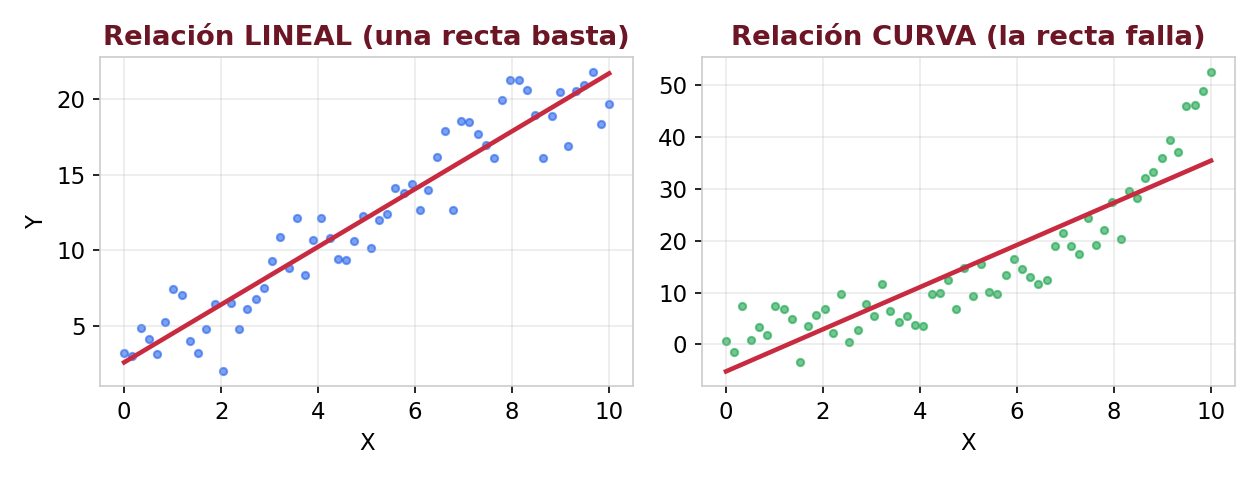
\includegraphics[width=\textwidth]{fig_lineal_vs_curva.png}
    \end{column}
    \begin{column}{0.42\textwidth}
      {\scriptsize\color{textMuted}
      \begin{itemize}\setlength{\itemsep}{5pt}
        \item[{\color{arcaRed}\scriptsize\faArrowRight}]
          \textbf{Declive de un pozo}: el primer año cae muchísimo; el quinto,
          casi nada. El paso \textbf{no} vale lo mismo.
        \item[{\color{arcaRed}\scriptsize\faArrowRight}]
          \textbf{Bombeo vs frecuencia}: sube al inicio y luego llega a una
          \textbf{meseta}: el pozo no da más.
        \item[{\color{arcaRed}\scriptsize\faExclamationTriangle}]
          En esos casos la correlación (que busca rectas) \textbf{subestima}
          la relación, y una recta la describe \textbf{mal}.
      \end{itemize}
      }
    \end{column}
  \end{columns}

  \vspace{4pt}
  {\scriptsize\color{textMuted}
    \faLightbulb[regular]\hspace{3pt}%
    Hoy empezamos por la \textbf{recta} porque es el modelo más simple de leer y explicar.
    Para lo curvo existen modelos más flexibles: los veremos en las próximas clases.}
\end{frame}

\begin{frame}{De la Relación a la Predicción}
  \vspace{-6pt}
  {\small\color{arcaDark}\bfseries
    Si la relación es firme y aproximadamente recta, la fórmula se vuelve una
    \textbf{máquina de responder}.}

  \vspace{10pt}
  \centering
  \begin{tikzpicture}[
    box/.style={rectangle, rounded corners=6pt, minimum width=4.6cm,
      minimum height=1.5cm, align=center, text=white, font=\small},
    arr/.style={-{Stealth[length=7pt]}, line width=1.6pt, arcaRed}]
    \node[box, fill=arcaDark] (a)
      {\faChartLine\hspace{4pt}\textbf{Describir} {\scriptsize(Módulo 2)}\\[3pt]{\scriptsize``DEN y AC: correlación \(-0.76\)''}};
    \node[box, fill=arcaRed, right=2.4cm of a] (b)
      {\faMagic\hspace{4pt}\textbf{Predecir} {\scriptsize(hoy)}\\[3pt]{\scriptsize``dame DEN \(=2.4\) y te doy AC \(\approx 84\)''}};
    \draw[arr] (a) -- (b) node[midway, above, font=\scriptsize\color{textMuted}] {la fórmula};
  \end{tikzpicture}

  \vspace{12pt}
  {\footnotesize\color{textMuted}
  \begin{itemize}\setlength{\itemsep}{5pt}
    \item[{\color{arcaRed}\scriptsize\faArrowRight}]
      Un \textbf{modelo} no es más que eso: la relación \textbf{escrita como fórmula},
      lista para usarse una y mil veces.
    \item[{\color{arcaRed}\scriptsize\faArrowRight}]
      \textbf{Machine Learning} = el computador \textbf{encuentra la fórmula} a partir
      de los ejemplos, en vez de que la programemos a mano.
    \item[{\color{codeGreen}\scriptsize\faCheck}]
      La usaremos para \textbf{rellenar el tramo del sensor dañado} --- sin re-loguear.
  \end{itemize}
  }
\end{frame}

\begin{frame}{Vocabulario de Machine Learning}
  \vspace{-6pt}
  {\small\color{arcaDark}\bfseries
    Dos palabras que usaremos todo el módulo:}

  \vspace{10pt}
  \begin{columns}[T]
    \begin{column}{0.48\textwidth}
      \centering
      {\Large\color{arcaRed}\faBullseye}\\[6pt]
      {\normalsize\bfseries\color{arcaDark} Target (objetivo)}\\[4pt]
      {\footnotesize\color{textMuted} Lo que queremos \textbf{predecir}.\\
      Se le dice también \texttt{y}.\\[4pt]
      Aquí: el sónico \texttt{AC}.}
    \end{column}
    \begin{column}{0.48\textwidth}
      \centering
      {\Large\color{arcaRed}\faSlidersH}\\[6pt]
      {\normalsize\bfseries\color{arcaDark} Features (variables)}\\[4pt]
      {\footnotesize\color{textMuted} Lo que usamos \textbf{para} predecir.\\
      Se les dice también \texttt{X}.\\[4pt]
      Aquí: \texttt{DEN, NEU, GR, RDEP}.}
    \end{column}
  \end{columns}

  \vspace{12pt}
  \centering
  {\footnotesize\color{arcaDark}
    Un modelo aprende la relación \quad
    \(\texttt{X} \;\longrightarrow\; \texttt{y}\) \quad
    a partir de los ejemplos.}
\end{frame}

%% ═════════════════════════════════════════════════════════════════════════════
\sectionframe{Los Datos}{El well log que vamos a usar}
% ═════════════════════════════════════════════════════════════════════════════
\begin{frame}[fragile,shrink=8]{El Dataset de Hoy: el Well Log de Volve}
  \vspace{-4pt}
  {\small\color{arcaDark}\bfseries
    El mismo pozo 15/9-19 de Volve que ya conocemos, ahora como tabla para modelar.}

  \vspace{4pt}
  \begin{columns}[T]
    \begin{column}{0.52\textwidth}
      \begin{pyblock}
import pandas as pd
reg = pd.read_csv(url)
reg.head()
      \end{pyblock}
      \vspace{2pt}
      \begin{outputblock}[]
    PROF    GR   DEN   NEU    AC
0  3550.2  55.8  2.17  51.2  54.6
1  3550.4  55.1  2.17  51.2  54.6
2  3550.5  56.1  2.17  51.2  54.6
      \end{outputblock}
    \end{column}
    \begin{column}{0.44\textwidth}
      {\scriptsize\color{textMuted}
      \begin{itemize}\setlength{\itemsep}{4pt}
        \item[{\color{arcaRed}\scriptsize\faTable}]
          \textbf{6\,893 filas}: cada una es una \textbf{profundidad}
          con todas sus mediciones.
        \item[{\color{arcaRed}\scriptsize\faColumns}]
          Ya está \textbf{limpio} (sin \texttt{NaN}) --- eso lo hicieron
          en el Módulo 2.
        \item[{\color{arcaRed}\scriptsize\faBullseye}]
          Queremos predecir la columna \texttt{AC} (el sónico).
      \end{itemize}
      }
    \end{column}
  \end{columns}
\end{frame}

\begin{frame}{¿Qué Mide Cada Columna? (1/2)}
  \vspace{-6pt}
  {\small\color{arcaDark}\bfseries
    Antes de modelar, entendamos las variables. Todas son mediciones físicas de la roca.}

  \vspace{4pt}
  \centering
  {\footnotesize
  \renewcommand{\arraystretch}{1.5}
  \begin{tabular}{@{}l l p{6.6cm}@{}}
    \toprule
    {\bfseries\color{arcaRed} Columna} & {\bfseries\color{arcaDark} Unidad}
      & {\bfseries\color{arcaDark} Qué mide} \\
    \midrule
    \rowcolor{arcaGray}
    \texttt{AC} \tiny(objetivo) & µs/ft
      & \textbf{Sónico}: cuánto tarda el sonido en cruzar la roca. Roca dura → rápido → AC bajo. \\
    \texttt{DEN} & g/cm\(^3\)
      & \textbf{Densidad}: qué tan pesada es la roca. \\
    \texttt{NEU} & \%
      & \textbf{Neutrón}: mide el hidrógeno de los fluidos → indica \textbf{porosidad}. \\
    \bottomrule
  \end{tabular}
  }

  \vspace{8pt}
  {\footnotesize\color{textMuted}
    \faLightbulb[regular]\hspace{4pt}%
    Nota: en otros softwares \texttt{DEN} y \texttt{NEU} aparecen como \texttt{RHOB} y \texttt{NPHI}.
    Es la misma medición, distinto nombre.}
\end{frame}

\begin{frame}{¿Qué Mide Cada Columna? (2/2)}
  \vspace{-6pt}
  \centering
  {\footnotesize
  \renewcommand{\arraystretch}{1.5}
  \begin{tabular}{@{}l l p{6.6cm}@{}}
    \toprule
    {\bfseries\color{arcaRed} Columna} & {\bfseries\color{arcaDark} Unidad}
      & {\bfseries\color{arcaDark} Qué mide} \\
    \midrule
    \texttt{GR} & GAPI
      & \textbf{Gamma Ray}: radioactividad natural. Alta en arcillas, baja en arenas limpias. \\
    \texttt{RDEP} & ohm·m
      & \textbf{Resistividad}: resistencia al paso de corriente. Alta = petróleo; baja = agua salada. \\
    \texttt{PROF} & m
      & \textbf{Profundidad}: dónde se tomó la medición (identifica la fila). \\
    \bottomrule
  \end{tabular}
  }

  \vspace{8pt}
  \begin{columns}[T]
    \begin{column}{0.48\textwidth}
      \begin{tcolorbox}[colback=arcaGray, colframe=codeGreen, boxrule=0pt,
        leftrule=3pt, arc=3pt, left=6pt, right=6pt, top=4pt, bottom=4pt]
        {\scriptsize\color{arcaDark}\bfseries\faBullseye\hspace{4pt}Target (lo que predecimos):}\\[2pt]
        {\scriptsize\color{textMuted} \texttt{AC} --- el sónico}
      \end{tcolorbox}
    \end{column}
    \begin{column}{0.48\textwidth}
      \begin{tcolorbox}[colback=arcaGray, colframe=arcaRed, boxrule=0pt,
        leftrule=3pt, arc=3pt, left=6pt, right=6pt, top=4pt, bottom=4pt]
        {\scriptsize\color{arcaDark}\bfseries\faSlidersH\hspace{4pt}Features (lo que usamos):}\\[2pt]
        {\scriptsize\color{textMuted} \texttt{DEN, NEU, GR, RDEP}}
      \end{tcolorbox}
    \end{column}
  \end{columns}
\end{frame}

\begin{frame}[fragile,shrink=18]{Explorar: ¿Qué Feature Predice Mejor?}
  \vspace{-4pt}
  {\small\color{arcaDark}\bfseries
    Calculamos la correlación de cada feature con el target. Nos dice por dónde empezar.}

  \vspace{4pt}
  \begin{columns}[T]
    \begin{column}{0.46\textwidth}
      \begin{pyblock}
reg.corr()["AC"]
      \end{pyblock}
      \vspace{2pt}
      \begin{outputblock}
DEN    -0.76
NEU     0.72
GR      0.36
RDEP   -0.10
      \end{outputblock}
    \end{column}
    \begin{column}{0.52\textwidth}
      \centering
      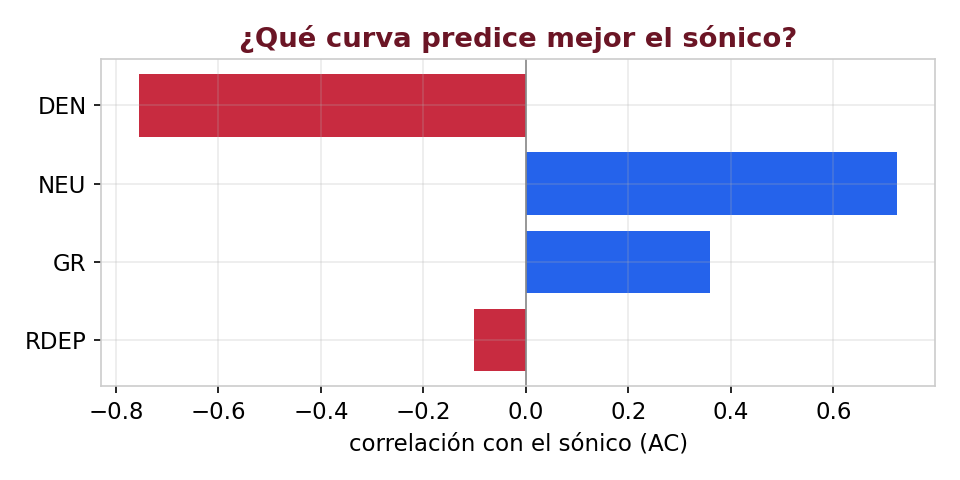
\includegraphics[width=\textwidth]{fig_explora_corr.png}
    \end{column}
  \end{columns}

  \vspace{4pt}
  {\scriptsize\color{textMuted}
  \begin{itemize}\setlength{\itemsep}{2pt}
    \item[{\color{codeGreen}\scriptsize\faCheck}]
      \texttt{DEN} y \texttt{NEU} son las más fuertes; \texttt{RDEP} casi no aporta.
    \item[{\color{arcaRed}\scriptsize\faArrowRight}]
      \texttt{DEN} negativo tiene sentido físico: roca más densa \(\to\) sonido más rápido \(\to\) sónico más bajo.
  \end{itemize}
  }
\end{frame}

%% ═════════════════════════════════════════════════════════════════════════════
\sectionframe{La Mejor Recta}{Regresión lineal simple}
% ═════════════════════════════════════════════════════════════════════════════
\begin{frame}{¿Cuál es la ``Mejor'' Recta? Los Residuos}
  \vspace{-6pt}
  {\small\color{arcaDark}\bfseries
    La mejor recta es la que pasa \textbf{más cerca} de todos los puntos.}

  \vspace{4pt}
  \begin{columns}[T]
    \begin{column}{0.52\textwidth}
      \centering
      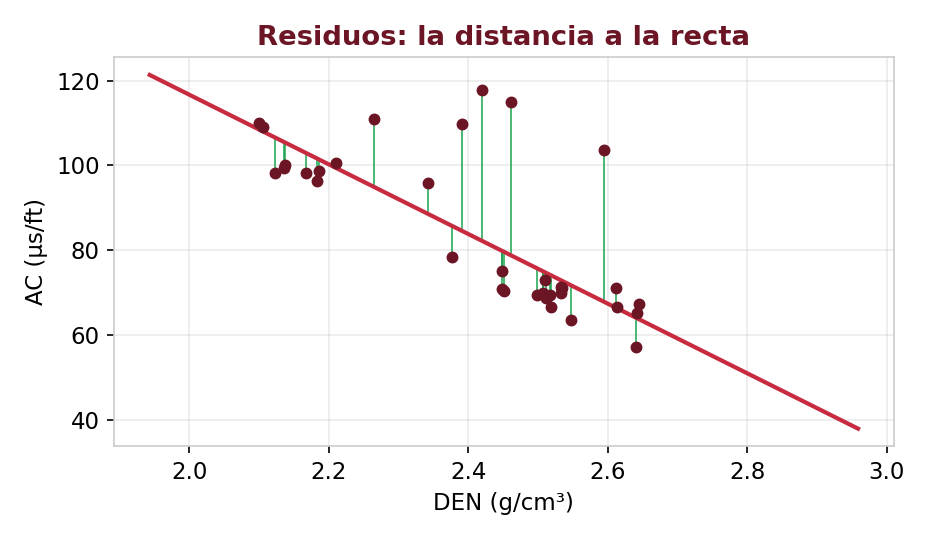
\includegraphics[width=\textwidth]{fig_residuos.png}
    \end{column}
    \begin{column}{0.44\textwidth}
      {\footnotesize\color{textMuted}
      \begin{itemize}\setlength{\itemsep}{6pt}
        \item[{\color{codeGreen}\scriptsize\faRulerVertical}]
          El \textbf{residuo} (verde) es el error: distancia entre
          el punto real y la recta.
        \item[{\color{arcaRed}\scriptsize\faArrowRight}]
          La mejor recta \textbf{minimiza} esos errores
          (los eleva al cuadrado y los suma: \textit{mínimos cuadrados}).
        \item[{\color{arcaRed}\scriptsize\faRobot}]
          \texttt{scikit-learn} encuentra esa recta óptima
          por nosotros.
      \end{itemize}
      }
    \end{column}
  \end{columns}
\end{frame}

\begin{frame}[fragile,shrink=26]{Nuestro Primer Modelo con scikit-learn}
  \vspace{-4pt}
  {\small\color{arcaDark}\bfseries
    \texttt{scikit-learn} (\texttt{sklearn}) es la librería de Machine Learning. Tres pasos y listo.}

  \vspace{4pt}
  \begin{columns}[T]
    \begin{column}{0.56\textwidth}
      \begin{pyblock}
from sklearn.linear_model import LinearRegression

X = reg[["DEN"]]     # feature
y = reg["AC"]        # target

modelo = LinearRegression()
modelo.fit(X, y)     # entrenar

print(modelo.intercept_, modelo.coef_)
      \end{pyblock}
      \vspace{2pt}
      \begin{outputblock}
280.9   [-82.1]
      \end{outputblock}
    \end{column}
    \begin{column}{0.40\textwidth}
      {\scriptsize\color{textMuted}
      \begin{itemize}\setlength{\itemsep}{4pt}
        \item[{\color{arcaRed}\scriptsize\faArrowRight}]
          \texttt{X} entre \textbf{corchetes dobles}: sklearn
          espera una tabla de features.
        \item[{\color{arcaRed}\scriptsize\faArrowRight}]
          \texttt{.fit(X, y)}: aquí el modelo \textbf{aprende}
          la mejor recta.
        \item[{\color{codeGreen}\scriptsize\faCheck}]
          Resultado: \(b=280.9\), \(m=-82.1\).
      \end{itemize}
      }
    \end{column}
  \end{columns}
\end{frame}

\begin{frame}[fragile,shrink=12]{Interpretar y Predecir}
  \vspace{-4pt}
  {\small\color{arcaDark}\bfseries
    El modelo aprendido es: \quad \(\texttt{AC} = 280.9 - 82.1 \times \texttt{DEN}\)}

  \vspace{6pt}
  \begin{columns}[T]
    \begin{column}{0.50\textwidth}
      {\scriptsize\color{arcaDark}\bfseries Leer el coeficiente:}
      \vspace{2pt}
      {\scriptsize\color{textMuted}
        Por cada \texttt{+1} g/cm\(^3\) de densidad, el sónico
        \textbf{baja 82} µs/ft. El signo negativo confirma la
        física: roca más densa, sonido más rápido.}

      \vspace{6pt}
      {\scriptsize\color{arcaDark}\bfseries Predecir un valor nuevo:}
      \begin{pyblock}
modelo.predict([[2.4]])
      \end{pyblock}
      \vspace{-2pt}
      \begin{outputblock}[]
[83.8]
      \end{outputblock}
    \end{column}
    \begin{column}{0.46\textwidth}
      \centering
      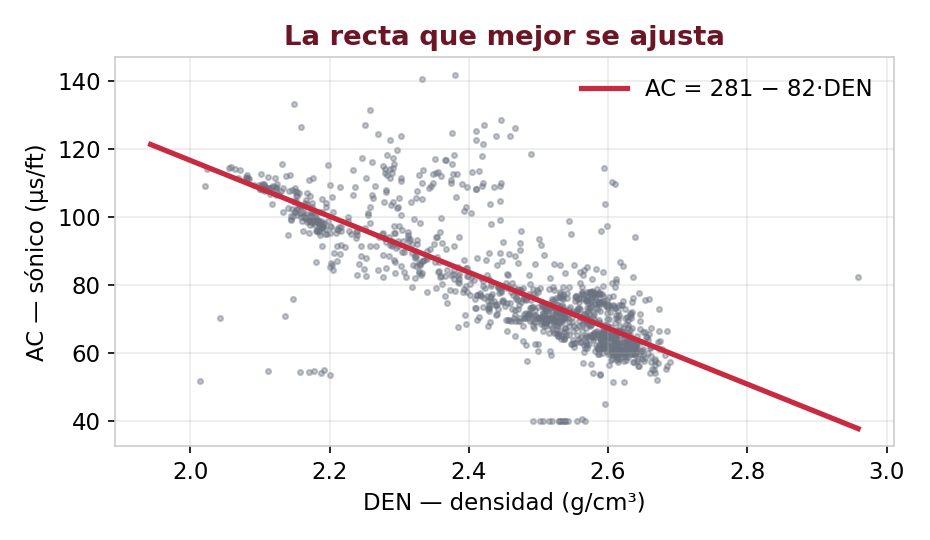
\includegraphics[width=\textwidth]{fig_reg_simple.png}
    \end{column}
  \end{columns}
\end{frame}

%% ═════════════════════════════════════════════════════════════════════════════
\sectionframe{¿Qué Tan Bueno es el Modelo?}{Las métricas de error}
% ═════════════════════════════════════════════════════════════════════════════
\begin{frame}{Medir el Error: RMSE y MAE}
  \vspace{-6pt}
  {\small\color{arcaDark}\bfseries
    Un modelo se juzga por su error: qué tan lejos caen las predicciones de la realidad.}

  \vspace{6pt}
  \begin{columns}[T]
    \begin{column}{0.48\textwidth}
      {\footnotesize\color{arcaDark}\bfseries\faRuler\hspace{4pt}MAE --- Error Absoluto Medio}
      \vspace{2pt}
      {\scriptsize\color{textMuted}
        El promedio de las distancias (sin signo). Fácil de leer:
        ``en promedio me equivoco por tanto''.}
    \end{column}
    \begin{column}{0.48\textwidth}
      {\footnotesize\color{arcaDark}\bfseries\faRulerCombined\hspace{4pt}RMSE --- Raíz del Error Cuadrático}
      \vspace{2pt}
      {\scriptsize\color{textMuted}
        Parecido, pero \textbf{castiga más} los errores grandes.
        Es la métrica más usada.}
    \end{column}
  \end{columns}

  \vspace{8pt}
  \centering
  \begin{tcolorbox}[colback=arcaGray, colframe=arcaRed, boxrule=0pt, leftrule=3pt,
    arc=3pt, left=8pt, right=8pt, top=5pt, bottom=5pt, width=0.8\textwidth]
    {\footnotesize\color{arcaDark}
      Ambas están en las \textbf{mismas unidades del target} (µs/ft).
      Entre más \textbf{bajas}, mejor. Un RMSE de 0 sería una predicción perfecta.}
  \end{tcolorbox}

  \vspace{4pt}
  {\scriptsize\color{textMuted}
    \faLightbulb[regular]\hspace{3pt}%
    ``RMSE = 11'' significa: mis predicciones del sónico se desvían, típicamente, unos 11 µs/ft del valor real.}
\end{frame}

\begin{frame}{R\textsuperscript{2}: ¿Mejor que Adivinar la Media?}
  \vspace{-6pt}
  {\small\color{arcaDark}\bfseries
    RMSE nos da un número, pero ¿11 es bueno o malo? R\textsuperscript{2} lo pone en contexto.}

  \vspace{4pt}
  \begin{columns}[T]
    \begin{column}{0.50\textwidth}
      \centering
      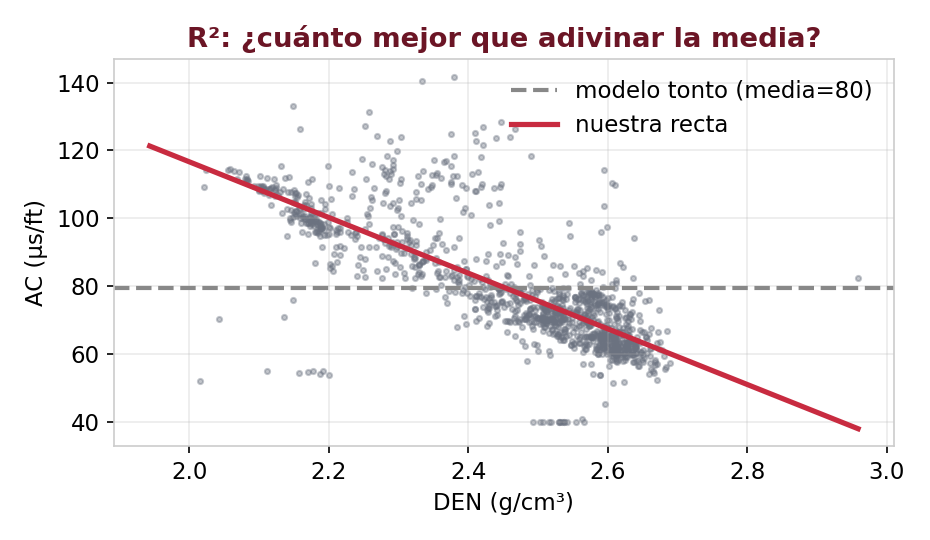
\includegraphics[width=\textwidth]{fig_r2_baseline.png}
    \end{column}
    \begin{column}{0.46\textwidth}
      {\footnotesize\color{textMuted}
      \begin{itemize}\setlength{\itemsep}{5pt}
        \item[{\color{arcaRed}\scriptsize\faArrowRight}]
          El \textbf{``modelo tonto''} siempre predice la media
          (la línea gris punteada).
        \item[{\color{arcaRed}\scriptsize\faArrowRight}]
          \textbf{R\textsuperscript{2}} mide cuánto \textbf{mejor} es nuestra recta
          que ese modelo tonto.
        \item[{\color{codeGreen}\scriptsize\faCheck}]
          \(R^2 = 1\): perfecto. \(R^2 = 0\): igual que la media.
          \textbf{Se lee como un porcentaje} de lo que el modelo explica.
      \end{itemize}
      }
    \end{column}
  \end{columns}
\end{frame}

\begin{frame}[fragile,shrink=30]{Las Métricas en Código}
  \vspace{-4pt}
  {\small\color{arcaDark}\bfseries
    sklearn las calcula por nosotros. Este es nuestro modelo simple (\texttt{AC} vs \texttt{DEN}).}

  \vspace{4pt}
  \begin{columns}[T]
    \begin{column}{0.56\textwidth}
      \begin{pyblock}
from sklearn.metrics import (
    mean_squared_error, r2_score)

pred = modelo.predict(X)

rmse = mean_squared_error(y, pred) ** 0.5
r2 = r2_score(y, pred)

print("RMSE:", rmse)
print("R2:", r2)
      \end{pyblock}
      \vspace{2pt}
      \begin{outputblock}
RMSE: 11.7
R2: 0.57
      \end{outputblock}
    \end{column}
    \begin{column}{0.40\textwidth}
      {\scriptsize\color{textMuted}
      \begin{itemize}\setlength{\itemsep}{5pt}
        \item[{\color{codeGreen}\scriptsize\faCheck}]
          \textbf{RMSE 11.7}: nos equivocamos \(\sim\)11.7 µs/ft
          en promedio.
        \item[{\color{codeGreen}\scriptsize\faCheck}]
          \textbf{R\textsuperscript{2} 0.57}: la densidad sola explica el
          \textbf{57\%} del sónico.
        \item[{\color{arcaRed}\scriptsize\faArrowRight}]
          ¿El otro 43\%? Otras variables.
          \textbf{Agreguemos más features.}
      \end{itemize}
      }
    \end{column}
  \end{columns}
\end{frame}

%

\begin{frame}[shrink=15]{¿Cuál Métrica Uso? Criterios y Valores Aceptables}
  \vspace{-6pt}
  {\small\color{arcaDark}\bfseries
    Ninguna métrica decide sola: cada una responde una pregunta distinta.}

  \vspace{5pt}
  \centering
  {\scriptsize
  \renewcommand{\arraystretch}{1.45}
  \begin{tabular}{@{}l p{4.4cm} p{4.8cm}@{}}
    \toprule
    {\bfseries\color{arcaRed} Métrica} & {\bfseries\color{arcaDark} Cuándo elegirla}
      & {\bfseries\color{arcaDark} Qué es ``aceptable''} \\
    \midrule
    \texttt{MAE} & comunicar el error típico en unidades
      del negocio; robusta a datos raros
      & júzguela contra la \textbf{tolerancia de ingeniería} del uso final \\
    \texttt{RMSE} & cuando los errores grandes cuestan caro
      (los castiga más); la estándar para comparar modelos
      & debe ser \textbf{mucho menor} que la desviación estándar del target
        (si RMSE \(\approx\) desv., el modelo no supera a la media) \\
    \texttt{R\textsuperscript{2}} & comunicar ``\% explicado'';
      comparar entre problemas distintos (no tiene unidades)
      & \(>0.8\) excelente \(\cdot\) 0.6--0.8 \textbf{útil en la industria}
        \(\cdot\) 0.4--0.6 débil \(\cdot\) \(<0.4\) insuficiente \\
    \bottomrule
  \end{tabular}
  }

  \vspace{7pt}
  {\scriptsize\color{textMuted}
  \begin{itemize}\setlength{\itemsep}{3pt}
    \item[{\color{codeGreen}\scriptsize\faCheck}]
      Nuestro modelo: R\textsuperscript{2} test = \textbf{0.66} (útil) y RMSE = \textbf{10.6}
      sobre un target que se mueve entre 40 y 149 (\(\approx\)10\,\% del rango).
    \item[{\color{arcaRed}\scriptsize\faExclamationTriangle}]
      Siempre reportadas \textbf{sobre el test}, nunca sobre el train.
    \item[{\color{arcaRed}\scriptsize\faArrowRight}]
      La decisión final no es estadística: es \textbf{¿cuánto cuesta equivocarse}
      en el uso que le daremos?
  \end{itemize}
  }
\end{frame}

% ═════════════════════════════════════════════════════════════════════════════
\sectionframe{De Una a Muchas Variables}{Regresión múltiple}
% ═════════════════════════════════════════════════════════════════════════════
\begin{frame}[fragile,shrink=26]{Muchas Features: Regresión Múltiple}
  \vspace{-4pt}
  {\small\color{arcaDark}\bfseries
    Una recta con \textbf{varias} features. El código casi no cambia: solo la lista de columnas.}

  \vspace{4pt}
  \begin{columns}[T]
    \begin{column}{0.54\textwidth}
      \begin{pyblock}
X = reg[["DEN", "NEU", "GR", "RDEP"]]
y = reg["AC"]

modelo = LinearRegression()
modelo.fit(X, y)

r2 = modelo.score(X, y)
print("R2:", r2)
      \end{pyblock}
      \vspace{2pt}
      \begin{outputblock}
R2: 0.66
      \end{outputblock}
    \end{column}
    \begin{column}{0.42\textwidth}
      {\scriptsize\color{textMuted}
      \begin{itemize}\setlength{\itemsep}{5pt}
        \item[{\color{arcaRed}\scriptsize\faArrowRight}]
          La ecuación ahora tiene \textbf{un coeficiente
          por feature}:\\
          \(\texttt{AC}=b+m_1\texttt{DEN}+m_2\texttt{NEU}+\ldots\)
        \item[{\color{codeGreen}\scriptsize\faArrowUp}]
          R\textsuperscript{2} sube de \textbf{0.57 a 0.66}:
          juntas explican más que la densidad sola.
      \end{itemize}
      }
    \end{column}
  \end{columns}
\end{frame}

\begin{frame}[fragile,shrink=12]{¿Cuál Variable Importa Más?}
  \vspace{-4pt}
  {\small\color{arcaDark}\bfseries
    Tentación: mirar los coeficientes y decir ``el más grande manda''. \textbf{Cuidado, es una trampa.}}

  \vspace{4pt}
  \begin{columns}[T]
    \begin{column}{0.50\textwidth}
      \begin{outputblock}[title={\small\faTerminal\hspace{6pt}coeficientes crudos}]
DEN    -55.99
NEU      0.43
GR       0.08
RDEP    -0.06
      \end{outputblock}
      \vspace{3pt}
      {\scriptsize\color{textMuted}
        ¿\texttt{DEN} importa 700 veces más que \texttt{NEU}?
        \textbf{No necesariamente.}}
    \end{column}
    \begin{column}{0.46\textwidth}
      {\footnotesize\color{textMuted}
      \begin{itemize}\setlength{\itemsep}{6pt}
        \item[{\color{arcaRed}\scriptsize\faBalanceScale}]
          Los coeficientes dependen de las \textbf{unidades}.
        \item[{\color{arcaRed}\scriptsize\faArrowRight}]
          \texttt{DEN} va de 2 a 3 (rango 1);
          \texttt{NEU} va de 0 a 100 (rango 100).
        \item[{\color{arcaRed}\scriptsize\faArrowRight}]
          Comparar coeficientes de escalas distintas
          \textbf{no es justo}.
        \item[{\color{codeGreen}\scriptsize\faLightbulb}]
          Solución: poner todas las features en la
          \textbf{misma escala}.
      \end{itemize}
      }
    \end{column}
  \end{columns}
\end{frame}

%% ═════════════════════════════════════════════════════════════════════════════
\sectionframe{Estandarización}{Poner todo en la misma escala}
% ═════════════════════════════════════════════════════════════════════════════
\begin{frame}{El Problema de las Escalas}
  \vspace{-6pt}
  {\small\color{arcaDark}\bfseries
    Nuestras features viven en mundos numéricos totalmente distintos.}

  \vspace{4pt}
  \begin{columns}[T]
    \begin{column}{0.56\textwidth}
      \centering
      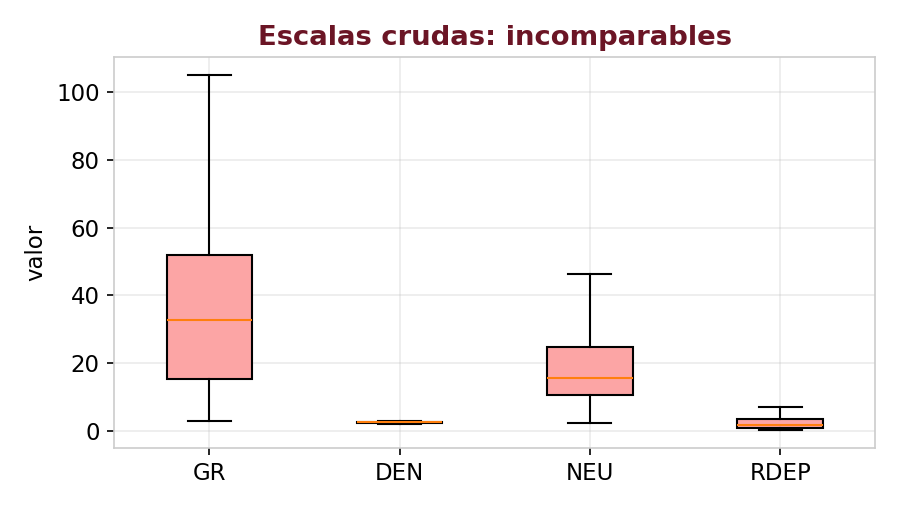
\includegraphics[width=\textwidth]{fig_escalas_antes.png}
    \end{column}
    \begin{column}{0.40\textwidth}
      {\footnotesize\color{textMuted}
      \begin{itemize}\setlength{\itemsep}{5pt}
        \item[{\color{arcaRed}\scriptsize\faArrowRight}]
          \texttt{GR} llega a 200, \texttt{NEU} a 100,
          \texttt{DEN} apenas se mueve entre 2 y 3.
        \item[{\color{arcaRed}\scriptsize\faArrowRight}]
          Para comparar su importancia --- y para muchos
          modelos --- esto es un problema.
        \item[{\color{codeGreen}\scriptsize\faLightbulb}]
          \textbf{Estandarizar}: reescalar todas para que
          sean comparables.
      \end{itemize}
      }
    \end{column}
  \end{columns}
\end{frame}

\begin{frame}[fragile,shrink=15]{El z-score y \texttt{StandardScaler}}
  \vspace{-4pt}
  {\small\color{arcaDark}\bfseries
    Estandarizar = a cada valor, restarle la media y dividir por la desviación. sklearn lo hace.}

  \vspace{4pt}
  \begin{columns}[T]
    \begin{column}{0.54\textwidth}
      \begin{pyblock}
from sklearn.preprocessing import StandardScaler

scaler = StandardScaler()
X_esc = scaler.fit_transform(X)
      \end{pyblock}
      \vspace{2pt}
      {\scriptsize\color{arcaDark}
        \(\displaystyle z = \frac{\text{valor} - \text{media}}{\text{desviación}}\)}
    \end{column}
    \begin{column}{0.42\textwidth}
      {\scriptsize\color{textMuted}
      \begin{itemize}\setlength{\itemsep}{5pt}
        \item[{\color{arcaRed}\scriptsize\faArrowRight}]
          Después, cada feature tiene \textbf{media 0} y
          \textbf{desviación 1}.
        \item[{\color{arcaRed}\scriptsize\faArrowRight}]
          Un valor de \texttt{+2} significa ``2 desviaciones
          por encima del promedio'', da igual la unidad
          original.
        \item[{\color{codeGreen}\scriptsize\faCheck}]
          Ya son \textbf{comparables}.
      \end{itemize}
      }
    \end{column}
  \end{columns}
\end{frame}

\begin{frame}{Ahora Sí: ¿Cuál Variable Importa Más?}
  \vspace{-6pt}
  {\small\color{arcaDark}\bfseries
    Con las features en la misma escala, los coeficientes ya se pueden comparar.}

  \vspace{4pt}
  \begin{columns}[T]
    \begin{column}{0.52\textwidth}
      \centering
      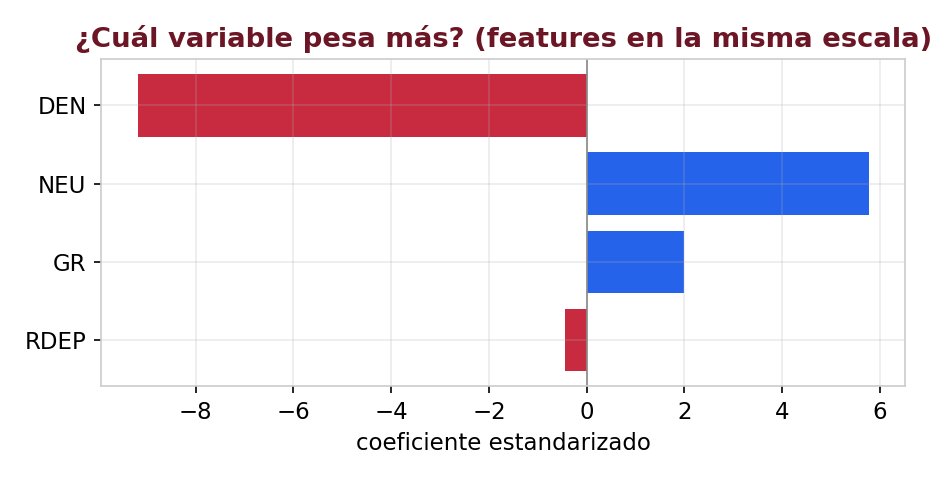
\includegraphics[width=\textwidth]{fig_coef.png}
    \end{column}
    \begin{column}{0.44\textwidth}
      {\footnotesize\color{textMuted}
      \begin{itemize}\setlength{\itemsep}{5pt}
        \item[{\color{codeGreen}\scriptsize\faTrophy}]
          \texttt{DEN} es la más influyente, seguida de
          \texttt{NEU}. Coincide con la física.
        \item[{\color{arcaRed}\scriptsize\faArrowRight}]
          \texttt{RDEP} casi no aporta --- como anticipó
          la correlación.
        \item[{\color{arcaRed}\scriptsize\faArrowRight}]
          Estandarizar no cambió el R\textsuperscript{2}; cambió nuestra
          \textbf{capacidad de interpretar}.
      \end{itemize}
      }
    \end{column}
  \end{columns}
\end{frame}

\begin{frame}{Una Trampa Silenciosa: Data Leakage}
  \vspace{-6pt}
  {\small\color{arcaDark}\bfseries
    Al estandarizar hay un error clásico que arruina la evaluación sin avisar.}

  \vspace{8pt}
  {\footnotesize\color{textMuted}
  \begin{itemize}\setlength{\itemsep}{8pt}
    \item[{\color{arcaRed}\Large\faTimesCircle}]
      \textbf{Mal:} estandarizar usando \textbf{todos} los datos, y
      luego separar en entrenamiento y prueba.\\
      {\scriptsize El scaler ``vio'' los datos de prueba → información filtrada → resultados
      demasiado optimistas.}
    \item[{\color{codeGreen}\Large\faCheckCircle}]
      \textbf{Bien:} \textbf{primero} separar, y ajustar el scaler
      \textbf{solo} con el entrenamiento.\\
      {\scriptsize El conjunto de prueba debe ser como datos ``del futuro'' que el modelo nunca vio.}
  \end{itemize}
  }

  \vspace{4pt}
  {\footnotesize\color{arcaDark}
    \faLightbulb[regular]\hspace{4pt}%
    Esto nos lleva a la idea más importante del día: \textbf{separar entrenamiento y prueba}.}
\end{frame}

%% ═════════════════════════════════════════════════════════════════════════════
\sectionframe{Train / Test Split}{¿Cómo sé si mi modelo sirve de verdad?}
% ═════════════════════════════════════════════════════════════════════════════
\begin{frame}{Una Pregunta Incómoda}
  \vspace{-6pt}
  {\small\color{arcaDark}\bfseries
    Medimos el R\textsuperscript{2} sobre los \textbf{mismos datos} con los que entrenamos. ¿Es eso confiable?}

  \vspace{10pt}
  \centering
  \begin{tcolorbox}[colback=arcaGray, colframe=arcaRed, boxrule=0pt, leftrule=3pt,
    arc=3pt, left=10pt, right=10pt, top=6pt, bottom=6pt, width=0.85\textwidth]
    {\footnotesize\color{arcaDark}\itshape
      Es como darle a un estudiante el examen \textbf{con las respuestas},
      dejarlo memorizarlas, y luego evaluarlo con \textbf{el mismo examen}.
      Sacará 100\ldots pero ¿de verdad aprendió?}
  \end{tcolorbox}

  \vspace{10pt}
  {\footnotesize\color{textMuted}
  \begin{itemize}\setlength{\itemsep}{5pt}
    \item[{\color{arcaRed}\scriptsize\faArrowRight}]
      Lo que importa es cómo predice sobre datos \textbf{que nunca vio}.
    \item[{\color{codeGreen}\scriptsize\faLightbulb}]
      Solución: \textbf{esconder una parte} de los datos antes de entrenar,
      y evaluar solo ahí.
  \end{itemize}
  }
\end{frame}

\begin{frame}[fragile,shrink=24]{\texttt{train\_test\_split}}
  \vspace{-4pt}
  {\small\color{arcaDark}\bfseries
    Partimos los datos: la mayoría para entrenar, una parte reservada para evaluar.}

  \vspace{4pt}
  \begin{columns}[T]
    \begin{column}{0.56\textwidth}
      \begin{pyblock}
from sklearn.model_selection import train_test_split

X_tr, X_te, y_tr, y_te = train_test_split(
    X, y, test_size=0.25, random_state=42)

modelo.fit(X_tr, y_tr)          # entrenar
print(modelo.score(X_te, y_te)) # evaluar
      \end{pyblock}
      \vspace{2pt}
      \begin{outputblock}
0.66
      \end{outputblock}
    \end{column}
    \begin{column}{0.40\textwidth}
      {\scriptsize\color{textMuted}
      \begin{itemize}\setlength{\itemsep}{4pt}
        \item[{\color{arcaRed}\scriptsize\faArrowRight}]
          \texttt{test\_size=0.25}: 75\% entrena, 25\% se reserva.
        \item[{\color{arcaRed}\scriptsize\faArrowRight}]
          \texttt{random\_state}: fija el sorteo para que sea
          \textbf{reproducible}.
        \item[{\color{codeGreen}\scriptsize\faCheck}]
          Entrenamos con \texttt{tr}, evaluamos con \texttt{te}:
          datos que el modelo \textbf{nunca vio}.
      \end{itemize}
      }
    \end{column}
  \end{columns}
\end{frame}

\begin{frame}{El Veredicto: Predicho vs Real en el Test}
  \vspace{-6pt}
  {\small\color{arcaDark}\bfseries
    La prueba de fuego: comparar predicciones contra la realidad en datos nuevos.}

  \vspace{4pt}
  \begin{columns}[T]
    \begin{column}{0.50\textwidth}
      \centering
      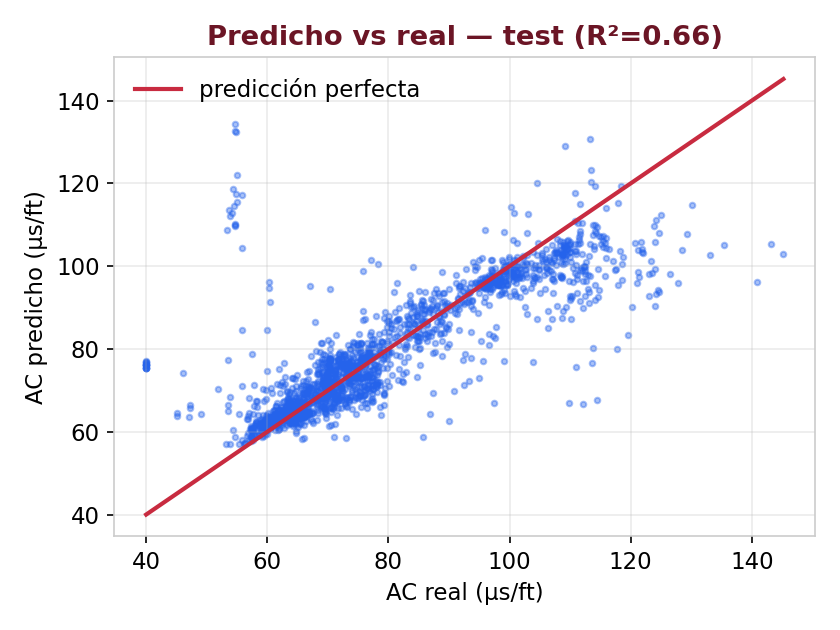
\includegraphics[width=0.92\textwidth]{fig_predicho_real.png}
    \end{column}
    \begin{column}{0.46\textwidth}
      {\footnotesize\color{textMuted}
      \begin{itemize}\setlength{\itemsep}{5pt}
        \item[{\color{arcaRed}\scriptsize\faArrowRight}]
          Cada punto: un tramo del pozo que el modelo
          \textbf{no usó} para entrenar.
        \item[{\color{codeGreen}\scriptsize\faCheck}]
          Caen cerca de la línea roja (predicción perfecta):
          el modelo \textbf{generaliza}.
        \item[{\color{arcaRed}\scriptsize\faArrowRight}]
          R\textsuperscript{2} en test \(\approx\) R\textsuperscript{2} en train (0.66 vs 0.67):
          \textbf{no memorizó}, aprendió.
      \end{itemize}
      }
    \end{column}
  \end{columns}
\end{frame}

\begin{frame}{Overfitting: Cuando el Modelo ``Memoriza''}
  \vspace{-6pt}
  {\small\color{arcaDark}\bfseries
    El síntoma se lee comparando el desempeño en entrenamiento vs en prueba.}

  \vspace{6pt}
  \centering
  {\footnotesize
  \renewcommand{\arraystretch}{1.5}
  \begin{tabular}{@{}l c c l@{}}
    \toprule
    {\bfseries\color{arcaDark} Situación} & {\bfseries\color{arcaDark} R\textsuperscript{2} train}
      & {\bfseries\color{arcaDark} R\textsuperscript{2} test} & {\bfseries\color{arcaDark} Diagnóstico} \\
    \midrule
    \rowcolor{arcaGray}
    Sano & 0.67 & 0.66 & {\color{codeGreen}Generaliza bien \faCheck} \\
    Overfitting & 0.98 & 0.55 & {\color{arcaRed}Memorizó, no aprendió} \\
    Underfitting & 0.30 & 0.29 & {\color{codeOrange}Demasiado simple} \\
    \bottomrule
  \end{tabular}
  }

  \vspace{8pt}
  {\footnotesize\color{textMuted}
  \begin{itemize}\setlength{\itemsep}{4pt}
    \item[{\color{arcaRed}\scriptsize\faArrowRight}]
      \textbf{Overfitting}: excelente en train, malo en test. El modelo
      memorizó el ruido en vez de la tendencia.
    \item[{\color{codeGreen}\scriptsize\faCheck}]
      Nuestro modelo está \textbf{sano}: por eso el train/test es
      imprescindible --- sin él no lo sabríamos.
  \end{itemize}
  }
\end{frame}

%% ═════════════════════════════════════════════════════════════════════════════
\sectionframe{Los Límites de la Recta}{Qué asume el modelo y cuándo se queda corto}
% ═════════════════════════════════════════════════════════════════════════════
\begin{frame}{Cuándo la Recta se Queda Corta}
  \vspace{-6pt}
  {\small\color{arcaDark}\bfseries
    Ejemplo real: predecir la producción de un pozo a lo largo del tiempo.}

  \vspace{4pt}
  \begin{columns}[T]
    \begin{column}{0.54\textwidth}
      \centering
      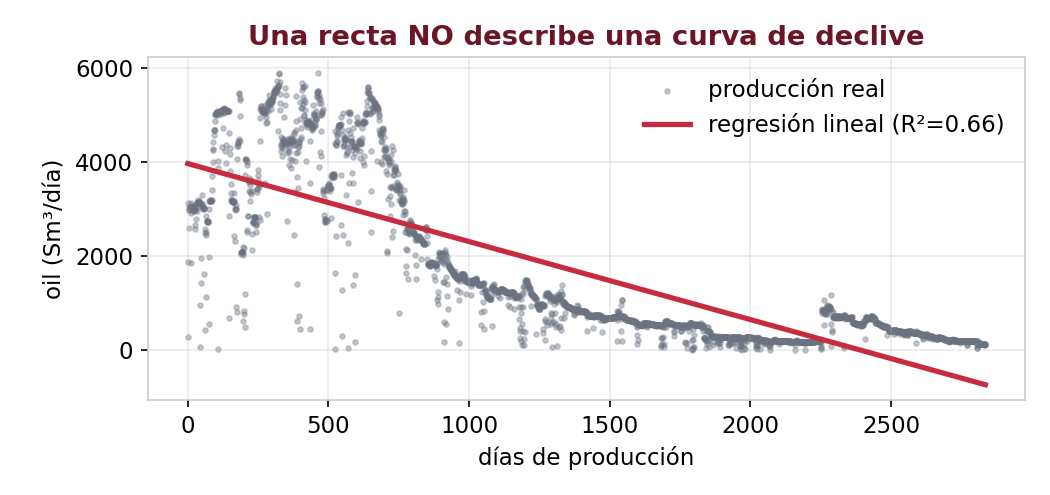
\includegraphics[width=\textwidth]{fig_no_lineal.png}
      {\scriptsize\color{textMuted}\itshape La curva de declive (Clase 3) no es una recta:
      la línea hasta predice producción \textbf{negativa}.}
    \end{column}
    \begin{column}{0.43\textwidth}
      {\scriptsize\color{arcaDark}\bfseries La regresión lineal asume:}
      \vspace{2pt}
      {\scriptsize\color{textMuted}
      \begin{itemize}\setlength{\itemsep}{3pt}
        \item[{\color{arcaRed}\scriptsize\faTimes}]
          \textbf{Linealidad}: el patrón es una recta.
        \item[{\color{arcaRed}\scriptsize\faTimes}]
          \textbf{Aditividad}: cada feature suma su efecto,
          sin que unas dependan de otras.
        \item[{\color{arcaRed}\scriptsize\faTimes}]
          \textbf{Sensible a outliers}: un dato raro tuerce la recta.
      \end{itemize}
      }
      \vspace{3pt}
      \begin{tcolorbox}[colback=arcaGray, colframe=codeGreen, boxrule=0pt,
        leftrule=3pt, arc=3pt, left=5pt, right=5pt, top=3pt, bottom=3pt]
        {\scriptsize\color{arcaDark}
        Cuando el patrón es curvo o complejo, se usan modelos
        \textbf{más flexibles} --- árboles, bosques, redes neuronales.
        \textbf{Los veremos en las próximas clases del módulo.}}
      \end{tcolorbox}
    \end{column}
  \end{columns}
\end{frame}

%% ═════════════════════════════════════════════════════════════════════════════
\sectionframe{Cierre}{Acaban de hacer Machine Learning}
% ═════════════════════════════════════════════════════════════════════════════
\begin{frame}{El Flujo que Aprendieron Hoy}
  \vspace{-4pt}
  \centering
  \begin{tikzpicture}[
    mlstep/.style={rectangle, rounded corners=5pt, fill=arcaGray, draw=arcaLightGray,
      minimum width=2.5cm, minimum height=1.15cm, align=center,
      font=\scriptsize, text=textDark},
    num/.style={circle, fill=arcaRed, text=white, font=\scriptsize\bfseries,
      minimum size=0.5cm, inner sep=0pt},
    ar/.style={-{Stealth[length=5pt]}, line width=1.2pt, arcaRed},
    node distance=0.55cm]
    \node[mlstep] (s1) {\faDatabase\\[2pt]Datos\\(X, y)};
    \node[mlstep, right=of s1] (s2) {\faCut\\[2pt]Train /\\Test};
    \node[mlstep, right=of s2] (s3) {\faBalanceScale\\[2pt]Estandarizar\\(solo train)};
    \node[mlstep, right=of s3] (s4) {\faRobot\\[2pt]Entrenar\\\texttt{.fit}};
    \node[mlstep, right=of s4] (s5) {\faChartLine\\[2pt]Evaluar\\(test)};
    \node[num, above=0.1cm of s1] {1}; \node[num, above=0.1cm of s2] {2};
    \node[num, above=0.1cm of s3] {3}; \node[num, above=0.1cm of s4] {4};
    \node[num, above=0.1cm of s5] {5};
    \draw[ar] (s1)--(s2); \draw[ar] (s2)--(s3); \draw[ar] (s3)--(s4); \draw[ar] (s4)--(s5);
  \end{tikzpicture}

  \vspace{10pt}
  {\footnotesize\color{textMuted}
  \begin{itemize}\setlength{\itemsep}{4pt}
    \item[{\color{codeGreen}\scriptsize\faCheck}]
      Este flujo es \textbf{el mismo} para casi todos los modelos del módulo:
      hoy fue regresión lineal, la semana entrante serán otros.
    \item[{\color{arcaRed}\scriptsize\faArrowRight}]
      Cambia el modelo (\texttt{LinearRegression} $\to$ otro), pero los pasos
      se mantienen.
  \end{itemize}
  }
\end{frame}

\begin{frame}{Lo Que Aprendimos Hoy}
  \vspace{-6pt}
  \begin{columns}[T]
    \begin{column}{0.48\textwidth}
      {\footnotesize\color{arcaDark}\bfseries Conceptos}
      \vspace{3pt}
      {\footnotesize\color{textMuted}
      \begin{itemize}\setlength{\itemsep}{2pt}
        \item[{\color{codeGreen}\scriptsize\faCheck}]
          Describir vs \textbf{predecir}; qué es un modelo
        \item[{\color{codeGreen}\scriptsize\faCheck}]
          Target y features (\texttt{X} $\to$ \texttt{y})
        \item[{\color{codeGreen}\scriptsize\faCheck}]
          Regresión lineal: la mejor recta (residuos)
        \item[{\color{codeGreen}\scriptsize\faCheck}]
          Métricas: RMSE, MAE, R\textsuperscript{2}
        \item[{\color{codeGreen}\scriptsize\faCheck}]
          Correlación, estandarización, data leakage
        \item[{\color{codeGreen}\scriptsize\faCheck}]
          Train/test y overfitting
        \item[{\color{codeGreen}\scriptsize\faCheck}]
          Los límites de la recta (linealidad)
      \end{itemize}
      }
    \end{column}
    \begin{column}{0.48\textwidth}
      {\footnotesize\color{arcaDark}\bfseries Herramientas (\texttt{sklearn})}
      \vspace{3pt}
      {\footnotesize\color{textMuted}
      \begin{itemize}\setlength{\itemsep}{2pt}
        \item[{\color{arcaRed}\scriptsize\faTools}]
          \texttt{LinearRegression} --- \texttt{.fit}, \texttt{.predict}, \texttt{.score}
        \item[{\color{arcaRed}\scriptsize\faTools}]
          \texttt{train\_test\_split}
        \item[{\color{arcaRed}\scriptsize\faTools}]
          \texttt{StandardScaler}
        \item[{\color{arcaRed}\scriptsize\faTools}]
          \texttt{r2\_score}, \texttt{mean\_squared\_error}
        \item[{\color{arcaRed}\scriptsize\faTools}]
          \texttt{df.corr()} para explorar
      \end{itemize}
      }
      \vspace{6pt}
      {\scriptsize\color{arcaDark}\itshape
        Logro del día: reconstruir un registro de pozo
        que costaría re-perforar para medir.}
    \end{column}
  \end{columns}
\end{frame}

% ─────────────────────────────────────────────────────────────────────────────
\begingroup
\setbeamertemplate{headline}{}
\setbeamertemplate{footline}{}
\setbeamertemplate{navigation symbols}{}
\begin{frame}[plain, noframenumbering]
  \begin{tikzpicture}[remember picture, overlay]
    \fill[arcaDark] (current page.south west) rectangle (current page.north east);
    \node[anchor=center, text=white, font=\Huge\bfseries]
      at ([yshift=1.5cm]current page.center) {¡Gracias!};
    \node[anchor=center, text=white!80, font=\large, text width=10cm, align=center]
      at ([yshift=0.2cm]current page.center)
      {Carlos Enrique Mosquera Trujillo};
    \node[anchor=center, text=white!60, font=\normalsize, text width=10cm, align=center]
      at ([yshift=-0.6cm]current page.center)
      {\faEnvelope\hspace{6pt}cmosquerat@unal.edu.co};
    \node[anchor=center, text=white!60, font=\normalsize, text width=10cm, align=center]
      at ([yshift=-1.3cm]current page.center)
      {Machine Learning for Petroleum Engineers Using Python};
    \node[anchor=center, text=white!40, font=\small]
      at ([yshift=-2.0cm]current page.center)
      {SLB Ecuador \quad$\cdot$\quad UDLA \quad$\cdot$\quad 2026};
  \end{tikzpicture}
\end{frame}
\endgroup

\end{document}
